\chapter{考察}
本章では,本研究で得られた知見について述べる.

\section{実験評価}
一連の実験を通して,AE特徴量を用いた特徴量拡張が,部分的には有効であることが示された.\\
特に,入力データを標準化して前処理したのち,オートエンコーダの隠れ層の構成を[20, 10, 5]とし,多数派クラスのみを学習データとしてオートエンコーダに学習させ,さらに生成したAE特徴量も標準化処理を行なった場合(表\ref{tab:lr-aes-majority-0},\ref{tab:rf-aes-majority-0},\ref{tab:svm-aes-majority-0},\ref{tab:lgb-aes-majority-0},\ref{tab:mp-aes-majority-0})に,平均的に最も精度が高く,特徴量拡張の効果が期待できると言える.
また,表\ref{tab:compare-dataset}にあるように,30個中25個のデータセットにおいて,最も高い精度を出したのは特徴量拡張をおこなったモデルであったことから,提案手法の有効性が示された.\\
しかしながら,その効果は微々たるものであり,確率的にはAE特徴量を加えない方が精度が良くなる可能性が高い.各データセットごと,オートエンコーダの構成ごとの精度の分布を図\ref{fig:compare-dataset}に示す.各グラフの横軸は,左から,AE特徴量なしのモデル,[20,10,5]の構成のオートエンコーダを用いたモデル,[20,10,5,10,20]の構成のオートエンコーダを用いたモデル,[20,10,5,10,5,10,20]の構成のオートエンコーダを用いたモデルである.縦軸は,各モデルの少数派クラスのF-accuracyである.\\
グラフからも,特徴量拡張による精度の差は,微々たるものであり,'car\_eval\_34','libras\_move','car\_eval\_4'や,'letter\_img'などは,特徴量拡張をしなかった方が精度が高いことがわかる.\\

比較的精度の高かった入力データを標準化したモデルのみでの各データセットごと,オートエンコーダの構成ごとの精度の分布を図\ref{fig:compare-dataset-std}に示す.標準化したものに限定すると,平均の精度が悪かった'car\_eval\_34','car\_eval\_4'や,'letter\_img'などのモデルが,特徴量拡張を適用したモデルで最も精度が高いことがわかる.\\
以上から,AE特徴量は標準化されたデータに対して高い効果を発揮することがわかる.\\

オートエンコーダに学習させるサンプルを多数派のクラスに限定することによってさらに精度の改善がなされた,これは,オートエンコーダが多数派の特徴を学習することにより,少数派クラスのデータを入力させたときに,多数派クラスのAE特徴量とは異なるユニークな特徴量を生成することができたからであると考えられる.\\
逆に少数派クラスのみを学習させたオートエンコーダでは,全てのデータを学習させたオートエンコーダよりも生成されたAE特徴量による特徴量拡張での精度改善は見られなかった.これは,少数派クラスのサンプル数が少ないために,少数派クラスの特徴を十分に学習することができなかった.あるいは,少数データに過学習されてしまい,多数派クラス・少数派クラスを問わず特異な特徴量を生成することができなかった可能性がある.\\

ハイパーパラメータチューニングを適応したモデルにおいては,30個のうち28のデータセットにおいて,最も高い精度を出したモデルが特徴量拡張を行なったモデルであった.
したがって,特徴量拡張を行なったモデルの方が,ハイパーパラメータチューニングの恩恵を受けやすいと言える.\\


\begin{figure}
    \centering
    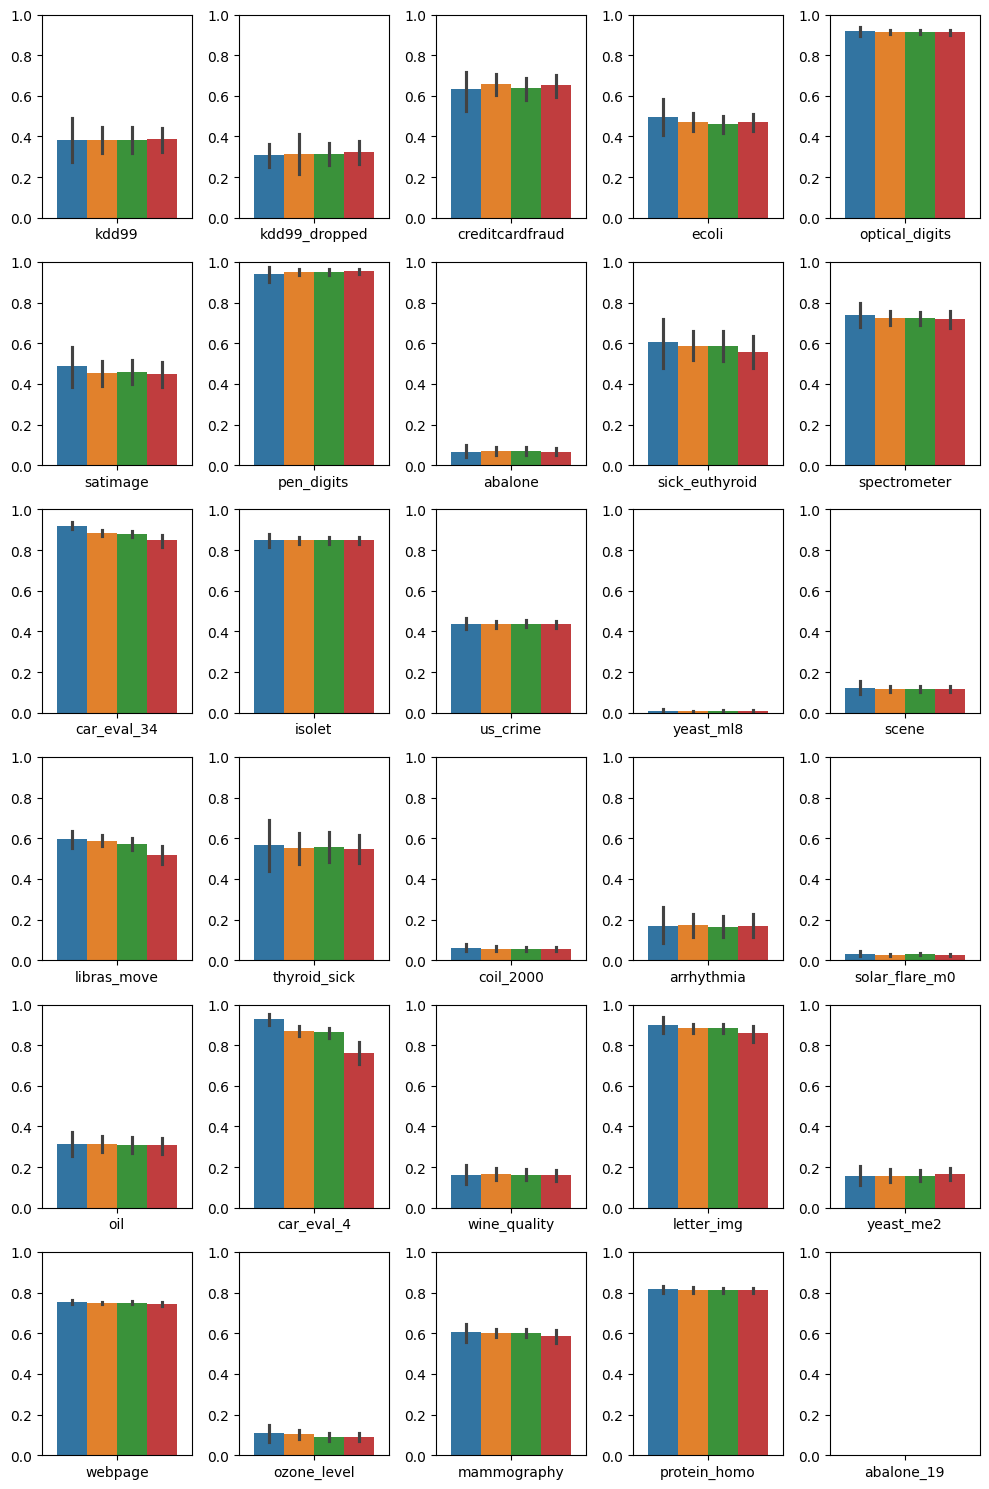
\includegraphics[width=0.8\textwidth]{figures/result-dataset.png}
    \caption{各データセットごと,オートエンコーダの構成ごとの精度の分布}
    \label{fig:compare-dataset}
\end{figure}

\begin{figure}
    \centering
    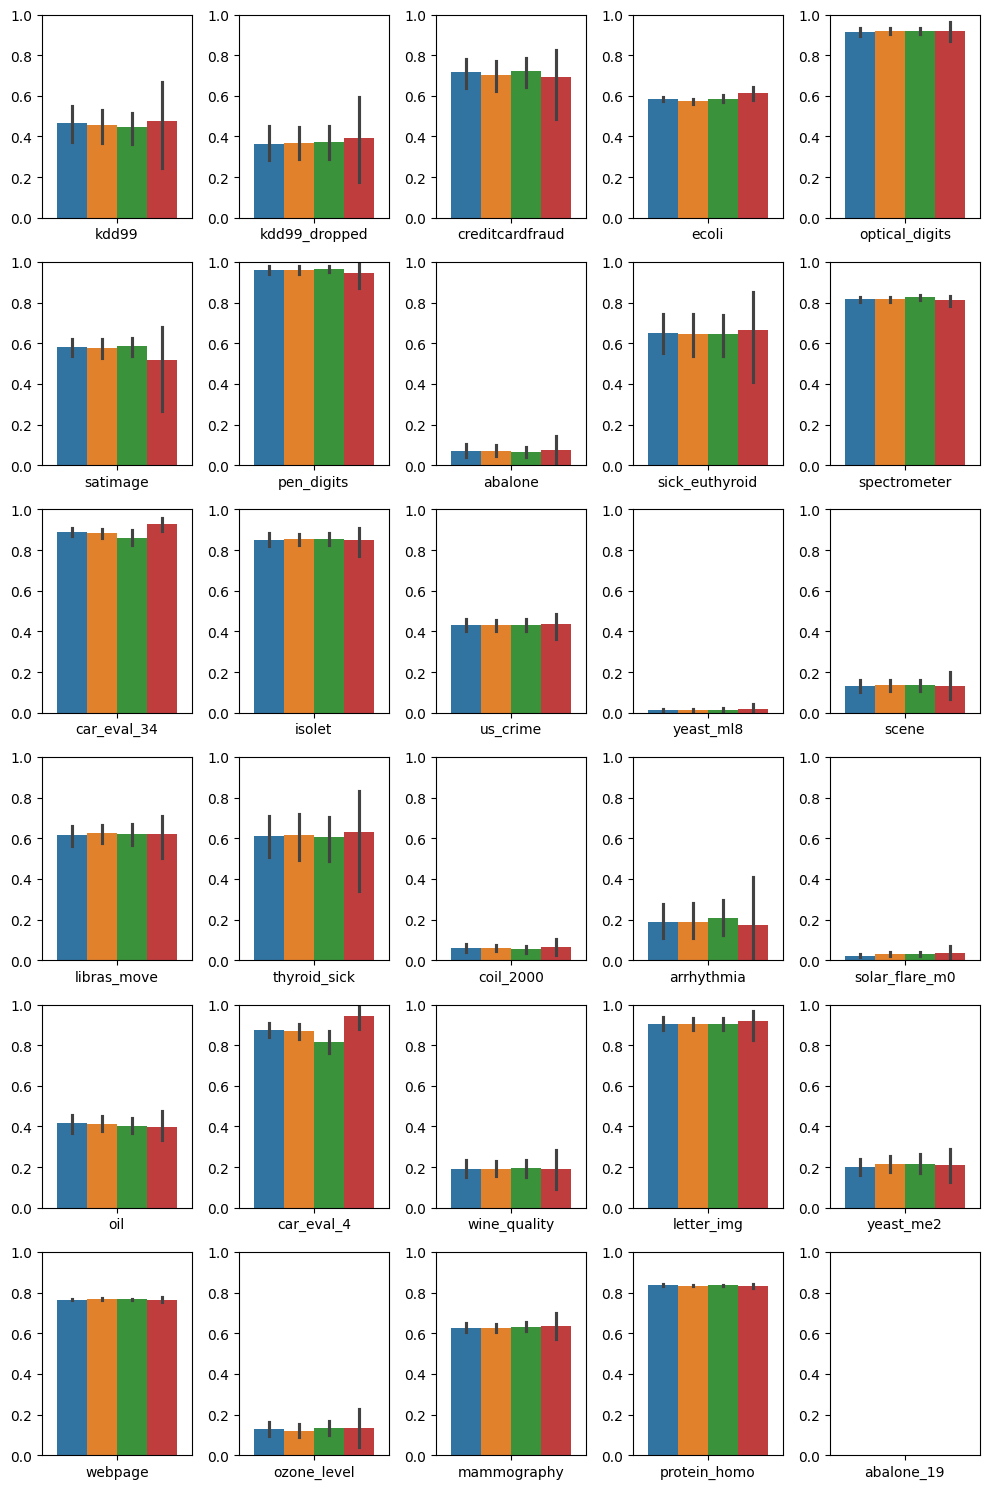
\includegraphics[width=0.8\textwidth]{figures/result-dataset-std.png}
    \caption{各データセットごと,オートエンコーダの構成ごとの精度の分布(標準化済み)}
    \label{fig:compare-dataset-std}
\end{figure}

\section{多重共線性の問題}
特徴量拡張を行なったモデルの中には,特徴量拡張を行なわなかったモデルよりも精度が低いものがあった.
その原因として,特徴量拡張により,特徴量同士の相関が高くなり,多重共線性が発生したことが考えられる.\\
多重共線性とは,複数の説明変数間に強い相関がある場合に生じる現象であり,回帰分析において,説明変数間の相関が高いと,回帰係数の推定値が不安定になる.\\